% 
%
\newgeometry{top=2cm, bottom=1cm, left=1cm, right=1cm,
               marginparsep=0cm, marginpar=0pt}
\newpage

\makeatletter
\cxset{bache scale/.store in = \scalebache@cx,
    bache left column width/.store in = \bacheleftcolumnwidth@cx,
    bache imagei/.store in = \bacheimagei@cx,
    bache imagei caption/.store in = \bacheimageicaption@cx,
    bache imageii/.store in = \bacheimageii@cx,
    bache imageii caption/.store in = \bacheimageiicaption@cx,
    bache left header/.store in = \bacheleftheader@cx,
    bache header/.store in = \bacheheader@cx}

\cxset{bache scale = 1,
    bache left column width = {\dimexpr\textwidth-.4\textwidth\relax},
    bache left header =,
    bache imagei = bache-01,
    bache imagei caption ={\begin{multicols}{2}\lorem\end{multicols}},
    bache imageii = nudeback,
    bache imageii caption = {JULES BACHE},
    bache header = \scalebox{.97}{THE DEAN OF US NUDE-PAINTERS}
    }
\newenvironment{bache}{%
\parindent0pt
\renewenvironment{leftcolumn}{%
   \minipage[t]{\bacheleftcolumnwidth@cx}%
   \leavevmode   
  }{\endminipage}\hspace*{0cm}%

 \renewenvironment{rightcolumn}{%
   \minipage[t][\textheight-45pt][t]{.37\textwidth}%
   \mbox{}%
  }{\endminipage}\hspace*{0cm}% 

\begin{minipage}[t][\textheight-35pt][t]{\scalebache@cx\textwidth}%
{\hrule\vbox to 0pt{\rule{1pt}{\textheight-35pt}}
\Large\bfseries\sffamily JULES BACHE GIVES HIS \$20,000,000 ART COLLECTION TO NEW YORK}\par%
\begin{leftcolumn}%
\mbox{}%ncessesary to line on top
\par\leavevmode\includegraphics[width=\linewidth]{\bacheimagei@cx}\par
\bacheimageicaption@cx%
\end{leftcolumn}\hfill%
\begin{rightcolumn}%
\mbox{}%
\intextsep0pt
\begin{wrapfigure}{l}{0pt}
 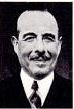
\includegraphics[width=3cm]{bache-02}
\caption*{\bfseries\sffamily \bacheimageiicaption@cx}
  \end{wrapfigure}\ignorespaces
 }
{\end{rightcolumn}%
\vfill
\end{minipage}} 

\begin{bache}
This layout has a dominant left column image. It is important to
ensure that the image has an aspect ratio to suit. Unfortunately
it is very difficult to crop and scale an image via \tex so a bit
of experimentation is appropriate.

It is also important to ensure that you add an adequate amount
of text during editing, otherwise the layout will not look very good. The right
column has two images (it really looks better when it has two images rather than
one and the bottom image is really a filler, if you have more or less
text you may have to go back and crop the image to suit. Any extra space on the right column is used as glue.

\vfill
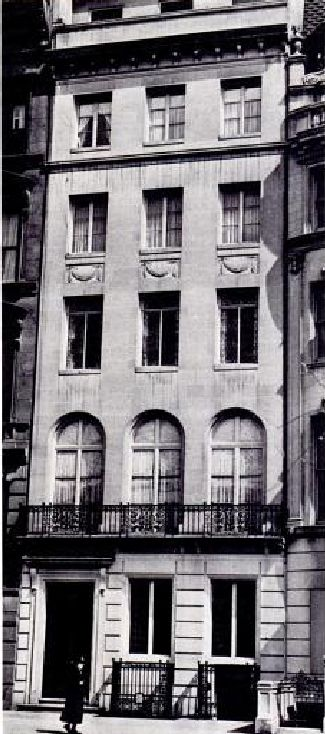
\includegraphics[width=\linewidth]{bache-03}
\end{bache}



\restoregeometry